\documentclass{kuisthesis}			% 特別研究報告書
\usepackage{listings,jlisting}
\usepackage{fancybox,ascmac}
\usepackage{amsmath}
\usepackage{tabularx}
\usepackage[dvipdfmx]{graphicx}
\usepackage{here}


\lstset{%listings の表示設定
breaklines = true,
tabsize = 2,
frame=shadowbox,
basicstyle = \small,
showstringspaces=false,
numbers=left,
framexleftmargin=8mm,
numberstyle=\scriptsize,
stepnumber=1,
numbersep=1zw,
language = Java}


\def\LATEX{{\rm (L\kern-.36em\raise.3ex\hbox{\sc a})\TeX}}
\def\LATex{\iLATEX\small}
\def\iLATEX#1{L\kern-.36em\raise.3ex\hbox{#1\bf A}\kern-.15em
    T\kern-.1667em\lower.7ex\hbox{E}\kern-.125emX}
\def\LATEXe{\ifx\LaTeXe\undefined \LaTeX 2e\else\LaTeXe\fi}
\def\LATExe{\ifx\LaTeXe\undefined \iLATEX\scriptsize 2e\else\LaTeXe\fi}
\let\EM\bf
\def\|{\verb|}
\def\<{\(\langle\)}
\def\>{\(\rangle\)}
\def\CS#1{{\tt\string#1}}

\jtitle[ IoT環境における状況依存型サービス連携の実現]%	% 和文題目(内容梗概/目次用)
	{ IoT環境における状況依存型サービス連携の実現}	% 和文題目
\etitle{Realization of situated service composition in IoT environment}	% 英文題目
\jauthor{渡辺 隆弘}				% 和文著者名
\eauthor{Takahiro Watanabe}			% 英文著者名
\supervisor{石田 亨 教授}			% 指導教員名
\date{平成28年2月6日}				% 提出年月日
\department{社会情報学}				% 修士論文の場合の専攻名

\begin{document}
\maketitle					% 「とびら」の出力

\begin{jabstract}				% 和文梗概
アブストラクト
研究の背景と、概要

研究の貢献
\begin{enumerate}
\item
Webとセンサーを繋ぐ画一化されたプラットフォームが存在しない
\item
Webサービスの利用にその都度リクエストを送信しなければならない
\item
サービス選択が手動
\end{enumerate}
\end{jabstract}
\begin{eabstract}				% 英文梗概
abstract

\end{eabstract}

\tableofcontents				% 目次の出力

\section{はじめに}\label{sec-intro}		% 本文の開始
はじめに
あいうえお

\section{関連研究}\label{sec-structure}
この章では本研究に利用している各用語についての説明を行う.

\subsection{IoT}\label{subsec-abstract}
IoT(Internet of Things)とは,様々な物理機器,建物,乗り物などにセンサーやソフトウェアを組み込むことで,情報交換やデータの収集を行えるネットワークを構築する仕組みである.以下のような例が考えられる.
\begin{itemize}
\item 離れた場所の環境を知る
温度,湿度,気圧.照度といった環境をセンサーによって知ることができる.
\item 物体の動きを知る
物体の動き(衝撃,振動,移動など)を知ることができる.
\item 物体の位置を知る
物体の位置(存在,通過など)を知ることができる.
\item 機器の制御を行う
空調の制御,照明の制御などを離れた場所から操作することができる.
\end{itemize}
このように,IoT環境下ではセンサーデータを用いた周囲の把握や,電気機器の利用,モニタリングが可能となり,より安全かつ快適な生活を実現できるようになる.\\
ここで,既存のIoTプラットフォームとして,OpenIoT\footnote{http://www.openiot.eu/}を取り上げる.OpenIoTはオープンソースで実装されているIoTプラットフォームである.OpenIoTではセンサーから取得したデータをミドルウェアを通じてデータベースに格納している.

\subsection{IoS}\label{subsec-abstract}
IoS(Internet of Service)とは,Webアプリケーションやサービスを組み合わせ,新たなサービスを構成するものである.Web上に点在するサービスを組み合わせ,より複雑な処理やサービス提供が可能となる.IoS基盤の例として言語グリッド\footnote{http://langrid.org/jp/}が挙げられる.言語グリッドは,辞書や機械翻訳などの言語資源が言語サービスとして登録され,共有可能とされているインターネット上の多言語サービス基盤である.多数の言語の相互翻訳,用例対訳,言語判別,音声認識,音声合成などのライブラリを,WebAPIから利用できる.

\subsection{CEP}
CEP(Complex Event Processing,または複合イベント処理)とは,刻々と生成されるデータをリアルタイムに処理するための方式である.事前に定義したルールに,リアルタイムにデータを挿入し,そのルールに応じて即座に処理を行う.これまでのビッグデータ分析の方法は,データをデータベースに蓄積し,任意のタイミングで参照し,分析するという手法であったために,情報の処理に時間がかかるという問題点があった.CEPは対象のデータを直近の範囲に絞り,メモリ上に読みこんで処理を行うため処理を高速化でき,”直近の数秒以内に”などの条件に沿ってデータを処理することが可能となる.本研究では,このCEPをストリーム形式であるセンサーデータに対し応用することを考える.

\subsection{サービス連携}
サービス連携とは,IoS基盤に集積された各原子サービスを組み合わせ,ユーザの要求を満たす高い品質(QoS,またはQuality of Service)の複合サービス(Composite Service)を構成する技術である.従来,複合サービスを構成するためには,ユーザが自らの要求を満足するような原子サービスを選択する方法が取られていた.また,複合サービスの自動構築を行う方法として,人工知能のプランニング技術を用いてワークフローを自動生成する研究が主流であった.しかし,IoS環境においては,同種の原子サービスが複数登録されるために,ワークフローを生成することよりむしろ,ワークフローに当てはめる原子サービスの選択が自動化できる必要がある.

\section{提案手法}
本章では,現状の課題を説明した後に,センサーのサービス化を行うための手法と,センサーから取得したデータによって,複合サービスのサービス選択,サービス実行を自動で行うための手法を提案する.

\subsection{課題点}
状況に応じたサービス選択を行うために,センサーから取得した情報によって複合サービスへの入力を変更することを考える.その際に以下の課題点が生じる.
\begin{enumerate}
\item センサーの仕様の不統一性\\
現状は同じ種類のセンサー(温度センサーや湿度センサーなど)でも,通信手段やデータフォーマットなどに差異がある.Webサービスを利用する際には,その場所に存在するセンサーから値を取得しサービスを実行するが,そのセンサーの仕様が統一されていなければ,それぞれのセンサーの仕様ごとにシステムの実装を行う必要が生まれる.
\item 複合サービス内の原子サービスの選択\\
これまで,複合サービス内の原子サービスの選択は,ユーザによって指定する方向で行われてきた.例えば,言語グリッドの翻訳サービスのうち,辞書翻訳を利用することを考える.言語グリッドの辞書翻訳には様々なサービスが登録されており,ユーザがどの辞書を用いるか指定する.\\
つまり,原子サービスの選択にユーザの知識や経験が要求されるため,以下のような問題点が生じる.
\begin{itemize}
\item ユーザが初めて複合サービスを利用する際にどのような原子サービスを利用すれば適当かが分からない
\item ユーザのサービスに対しての知識が不足しているために,ユーザのサービス選択がユーザの要求に関わらず固定化されてしまい,ユーザの要求を満たすよりよい原子サービスの組み合わせがあるにもかかわらず,より質の低いサービス選択を行ってしまう
\end{itemize}
\item 複合サービスのリアルタイム実行\\
複合サービスは,複数のWebサービスを組み合わせたものであるため,実行の仕様はWebサービスに基づく.Webサービスはリクエストに応じてレスポンスを返す形式であるため,Webサービスを利用するためには,ユーザはWebサービスにリクエストを送信する必要がある.
\end{enumerate}
これらの課題点を解決するために,以下の3つの手法を提案する.

\subsection{センサーのサービス化手法}
本節では,センサーのサービス化手法を提案する.現状は,前述した通りセンサーの仕様が画一化されていないために,センサーを利用するシステムを実装する際,センサーの種類によって異なる実装が必要であるという問題点が存在する.この問題点を本提案は解決する.
\\
データ定義をOpenIoTのセンサー定義に基づいて画一化する.OpenIoTのセンサー定義の例は以下であり,Observationオブジェクトとして実装される.データの値,取得時間や,温度,湿度,照度といったデータタイプを示すpropertyTypeなどが存在する.\\
\\
センサー定義例
\begin{lstlisting}
//Observation

	private String id;	
	private Date times;	
	private String sensorId;
	private String featureOfInterest=""; 
	private ArrayList<ObservedProperty> readings;
	private String metaGraph;
	private String dataGraph;
	
	
//ObservedProperty

	private static final long serialVersionUID = 1L;
	private Object value;
	private Date times;
	private String propertyType;
	private String unit;
	private String observationId;
\end{lstlisting}

センサーの開発者は,センサーから値を取得した際に,Observationを作成し,各変数に取得した値を格納するようにサービスを構成する.システム開発者はこのサービスの仕様に従ってシステムを実装することで,ユーザからは種々のセンサー間の違いは隠蔽され,画一化されたセンサーサービスとしてデータを利用することができる.例えば,センサーから温度20℃,湿度50\%のデータを取得した際には以下のようにObservationを生成する.\\
\\
Observation生成例
\begin{lstlisting}
Observation o = new Observation();    //Observationオブジェクトの作成
ArrayList<ObservedProperty> readings = new ArrayList<ObservedProperty>();     //ObservedPropertyのリストの作成
ObservedProperty tempProperty = new ObservedProperty();    //ObservedPropertyオブジェクトの作成
ObservedProperty humdProperty = new ObservedProperty();    
tempProperty.setPropertyType("http://openiot.eu/ontology/ns/AirTemperature");     //propertyTypeの設定
humdProperty.setPropertyType("http://openiot.eu/ontology/ns/AtmosphereHumidity");
tempProperty.setValue(20);    //valueに値を格納
humdProperty.setValue(50);
readings.add(tempProperty);     //ObservedPropertyのリストに追加
readings.add(humdProperty);
o.setReadings(readings);;    //Observationに作成したリストを格納
\end{lstlisting}



\subsection{状況依存型サービス選択手法}
本節では,センサーの値によって複合サービス中の原子サービスを選択する手法を提案する.センサーから取得した値をイベントエンジンによって処理することによってこの手法は実現される.詳細を以下に述べる.

\subsubsection{データの取得}
前節に基づいて作成されたセンサーサービスオブジェクトがサーバーへ送信される.サーバーはデータを受け取った時点で,このオブジェクトをCEPエンジンに挿入する.

\subsubsection{原子サービスの選択}
原子サービスの選択においては,ECAルールを応用することを考える.ECAルールとは,〜〜するものであり,
\begin{description}
\item[E] : Event
\item[C] : Condition
\item[A] : Action
\end{description}
の3つの状態が定義される.イベントが発生した際,その状況に応じてアクションを実行する,というルールの実行を行う.\\
本研究では,ECAルールをCEPエンジンで実現する.つまり,ECAルールを以下のように適用する.
\begin{description}
\item[E] : センサーからのデータの取得
\item[C] : センサーから取得した値
\item[A] : 選択するサービスとサービスへの入力の生成,サービスの実行
\end{description}
以上から,センサーからデータを取得した際,サーバーからCEPエンジンにデータを挿入し,事前に定義されたルールに基づいて,選択するサービスとサービスへの入力の生成とサービスの実行を行うという一連の処理が実行される.また,本研究ではCEPエンジンにおいて適用するルールは事前に定義されているものとし,状況に応じてどのような処理を実行すべきかというルールの構成の点についての議論は行わない.\\
この手法により以下の2点の問題点が解決される.
\begin{enumerate}
\item 複合サービス内の原子サービスの選択\\
ユーザがサービス選択を行わなければならないという問題点が存在した.一方,本提案では,専門家が一度ルールを作成すれば,センサーの値によって分岐するルールに従って原子サービスの選択を行うことができ,サービス連携においてユーザのサービスに対しての知識や経験に関わらず一定の質の高いサービス合成が可能となる.
\item 複合サービスのリアルタイム実行\\
サービス実行のためにユーザはWebサービスにリクエストを送信する必要があった.一方,本提案では,センサーの値をイベントとしてCEPエンジンに挿入し,リアルタイムで処理,アクションとして複合サービスへの入力生成とサービス実行を行うことによって,ユーザがサービスのリクエストを送信することなく,リアルタイムかつ自動的なサービス実行が可能となる.
\end{enumerate}

\section{提案アーキテクチャ}
本章では,前章に説明した提案手法に基づいて,IoT環境下で複合サービスの選択,実行を行うアーキテクチャの提案を行う.アーキテクチャは大きく

\subsection{アーキテクチャ図}
\begin{figure}[H]
 \begin{center}
  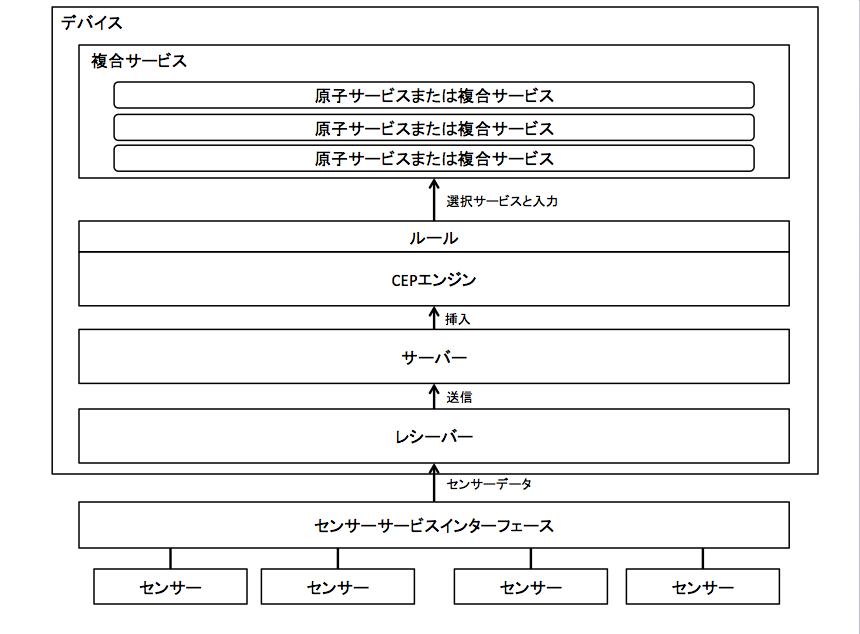
\includegraphics[width=\linewidth]{pic/architect.png}
  \caption{アーキテクチャ図}
 \end{center}
\end{figure}

\subsection{センサーサービスインターフェース}

\subsection{サーバー}

\subsection{CEPエンジン}

\subsection{複合サービス}

\section{実装}
本章では,前章に提案したアーキテクチャの実装について説明し,動作確認と評価について述べる.最後に実装の結果に対して考察を行う.
\subsection{シチュエーション}
体育館を利用するユーザに,温度,湿度などの情報から運動への助言を音声で与えるシステムを実装することを考える.ユーザは様々な言語圏のユーザが想定されるため,それぞれのユーザが利用する言語に基づいてアナウンスを行う必要がある.

\subsection{仕様}
言語はJavaを用いて実装した.以下に各モジュールの詳細を述べる.
\subsubsection{センサーデバイス}
体育館に設置することを想定するセンサーデバイスは,(株)オムロンの環境センサー\footnote{http://www.omron.co.jp/ecb/products/sensor/special/environmentsensor/}とする.このセンサーによって取得できるデータタイプの中から,今回は温度データと湿度データを利用する.
\subsubsection{ユーザデバイス}
ユーザが所持している端末を,iOSを搭載した端末とした.この端末はセンサーデバイスからデータを取得し, Observationを形成してサーバーへ送信するデバイスとして働く.センサーデバイスと本デバイス間の通信はBLE(Bluetooth Low Energy)を使用する.BLEは省電力の無線通信技術であり..... \\
構成要素は以下.
\begin{itemize}
\item WaikikiSensor\\
取得したデータを端末上に表示する.
\item Myviewcontrollor\\
データを取得し,センサーデータオブジェクトを構成してサーバに送信する.オブジェクトの構成法は3.1節で説明した方法に基づく.
\begin{enumerate}
\item Observationオブジェクトを生成する.
\item ObservedPropertyとしてtempProperty,humdPropertyを作成する.それぞれ,温度のデータ,湿度のデータを格納するオブジェクトである
\item ObservedPropertyそれぞれに,データタイプを示すPropertyTypeとデータの値を格納する.
\item tempPropertyとhumdPropertyをObservationオブジェクトに格納する.
\end{enumerate}
\end{itemize}
\subsubsection{サーバー}
サーバーと周辺のモジュールについて説明する.\\
以下のモジュールからなる.\\
\begin{itemize}
\item サーバー\\
サーバーはObservationReceiverクラスとして実装される.デバイスからObservationオブジェクトが送信された際に,CEPエンジンにでデータをイベントとして挿入する.
\item CEPエンジン\\
CEPエンジンとして,Javaで実装されたイベントエンジンであるDrools\footnote{https://www.drools.org/}を利用する.ルールとして"badminton.drl"を実装した.ルールの概要を表\ref{tab:drl}に挙げる.ルールは温度と湿度,ユーザの使用言語に加えWBGT(湿球黒球温度)によって定義される.本実装はWBGTを,
\begin{equation}
WBGT = \begin{cases}
T + (H - 80)/5 & (80 \leq H) \\
T -(80 -H)/5 & (H < 80)
\end{cases}
\end{equation}
\begin{flushright}
T:temperature(℃),H:humidity(\%)
\end{flushright}
と温度と湿度の値から近似して求める.

\begin{table}[p]
  \begin{center}
    \caption{badminton.drl}
    \begin{tabularx}{\linewidth}{|c|c|X|} \hline
      ルール名 & 条件 & 出力 \\ \hline \hline
      WBGCcalc1 & H $\geq$ 80 & WBGTの計算 WBGT $=$ T + (H - 80)/5  \\
      & & Propertytypeの作成:WBGT,Temperature \\
      & & Humidity,targetlanguageについて \\ 
      & & 再構成したObservationの再挿入 \\ \hline
      WBGCcalc2 & H $<$  80 & WBGTの計算 WBGT $=$ T - (80 - H)/5  \\
      & & Propertytypeの作成:WBGT,Temperature \\
      & & Humidity,targetlanguageについて \\ 
      & & 再構成したObservationの再挿入 \\ \hline \hline
      \multicolumn{3}{|c|}{イベントの再挿入後,テキストと利用サービスを} \\
      \multicolumn{3}{|c|}{Webサービスへの入力としたルールが実行される} \\ \hline \hline
      Phase & \multicolumn{2}{c|}{辞書翻訳(スポーツ辞書)サービスと音声合成サービスを} \\
      ルール & \multicolumn{2}{c|}{利用し,運動中のユーザへの注意喚起を行う} \\ \hline \hline
      Phase5 & WBGT $\geq$ 31  & 入力: "運動を中止しましょう."\\ \hline
      Phase4 & 28 $\leq$ WBGT $<$ 31 & 入力: "激しい運動は避け、積極的に休息と水分補給を行いましょう."\\ \hline
      Phase3 & 25 $\leq$ WBGT $<$ 28 & 入力: "激しい運動を行う際は,30分おきくらいに休息をとりましょう."\\ \hline
      Phase2 & 21 $\leq$ WBGT $<$ 25 & 入力: "水分補給には十分気をつけましょう."\\ \hline
      Phase1 & WBGT $<$ 21 & 入力: "熱中症の危険は少ないですが,適宜水分補給をしましょう."\\ \hline \hline
      Shuttle & \multicolumn{2}{c|}{辞書翻訳(バドミントン辞書)サービスと音声合成サービスを} \\
      ルール & \multicolumn{2}{c|}{利用し,シャトルコックの選択に関する情報を与える} \\ \hline \hline
      shuttle1 & T $\geq$ 33 & 入力:"1番のシャトルを使いましょう." \\ \hline 
      shuttle2 & 27 $\leq$ T $<$ 33 & 入力:"2番のシャトルを使いましょう."  \\ \hline
      shuttle3 & 22 $\leq$ T $<$ 27& 入力:"3番のシャトルを使いましょう."  \\ \hline
      shuttle4 & 17 $\leq$ T $<$ 22 & 入力:"4番のシャトルを使いましょう."  \\ \hline
      shuttle5 & 12 $\leq$ T $<$ 17 & 入力:"5番のシャトルを使いましょう."  \\ \hline
      shuttle6 & T $<$ 12 & 入力:"6番のシャトルを使いましょう." \\ \hline \hline
    \end{tabularx}
    \label{tab:drl}
  \end{center}
\end{table}

\begin{table}[htb]
    \begin{tabularx}{\linewidth}{|c|c|X|} \hline
      ルール名 & 条件 & 出力 \\ \hline \hline
      Strings & \multicolumn{2}{c|}{辞書翻訳(バドミントン辞書)サービスと音声合成サービスを} \\
      ルール & \multicolumn{2}{c|}{利用し,ラケットのストリングスに関する情報を与える} \\ \hline \hline
      strings1 & T $>$ 25 & "適正温度のときより+1ポンドのガットが適切です."  \\ \hline
      strings2 & 15 $\leq$ T $\leq$ 25 & "適正" \\ \hline
      strings3 & T $<$ 15 & "適正温度のときより-1ポンドのガットが適切です." \\ \hline
      floor & \multicolumn{2}{c|}{辞書翻訳(スポーツ辞書)サービスと音声合成サービスを} \\
      ルール & \multicolumn{2}{c|}{利用し,体育館の床面の結露による転倒を警告する} \\ \hline \hline
      floor & H $\geq$ 90 & "湿度が高く床が滑りやすくなっています.気をつけましょう." \\ \hline
    \end{tabularx}
\end{table}


\item 複合サービス\\
複合サービスとして,言語グリッドを利用する.言語グリッドは,登録された言語サービスを自由に組み合わせて新しい言語サービスを生み出す複合サービスである.本研究では,言語グリッドに登録されているサービスの中から,形態素解析サービスと辞書翻訳サービス,音声合成サービスを利用する.仕様は”URL”
\begin{itemize}
\item 形態素解析
\item 辞書翻訳
\item 音声合成
\end{itemize}
\end{itemize}


\subsection{動作確認}
\subsection{考察}





\section{終わりに}

\acknowledgments				% 謝辞
本研究を行うにあたり,貴重な資料をご提供いただきました株式会社オムロン様に深く感謝申し上げます.そして本研究を行うにあたり,熱心なご指導,ご助言を賜りました石田亨教授に厚く御礼申し上げます.また,日頃より数々のご助言をいただきました中口孝雄特定研究員,林冬惠助教をはじめ,石田・松原研究室の皆様方に心より感謝いたします.

\nocite{*}
\bibliographystyle{kuisunsrt}			% 文献スタイルの指定
\bibliography{guide}				% 参考文献の出力

						% 付録の開始
\Appendix[付録]
実装のソースコードを添付する.

\section{デバイスでセンサーデータを取得し、サーバーへ送信するモジュールのソースコード}
\subsection{MyviewController.java}
\lstinputlisting{/Users/admin/Documents/OpenIoT_integration/waikikisens/src/main/java/org/langrid/waikiki/sensor/MyviewController.java}

\subsection{WaikikiSensor.java}
\lstinputlisting{/Users/admin/Documents/OpenIoT_integration/waikikisens/src/main/java/org/langrid/waikiki/sensor/WaikikiSensor.java}

\section{受信したデータをルールエンジンに挿入し、状況に応じた出力を得るモジュールのソースコード}

\subsection{ObservationReceiverImpl.java}
\lstinputlisting{/Users/admin/Documents/OpenIoT_integration/waikikiws/src/main/java/org/langrid/waikikiws/service/ObservationReceiverImpl.java}

\subsection{Translator.java}
\lstinputlisting{/Users/admin/Documents/OpenIoT_integration/waikikiws/src/main/java/org/langrid/waikikiws/service/Translator.java}

\subsection{Binding.java}
\lstinputlisting{/Users/admin/Documents/OpenIoT_integration/waikikiws/src/main/java/org/langrid/waikikiws/Bindings.java}

\subsection{DroolsManager.java}
\lstinputlisting{/Users/admin/Documents/OpenIoT_integration/waikikiws/src/main/java/org/langrid/waikikiws/DroolsManager.java}

\subsection{DroolsUtil.java}
\lstinputlisting{/Users/admin/Documents/OpenIoT_integration/waikikiws/src/main/java/org/langrid/waikikiws/DroolsUtil.java}

\subsection{TargetLanguage}
\lstinputlisting{/Users/admin/Documents/OpenIoT_integration/waikikiws/src/main/java/org/langrid/waikikiws/service/TargetLanguage.java}

\subsection{VoiceText.java}
\lstinputlisting{/Users/admin/Documents/OpenIoT_integration/waikikiws/src/main/java/org/langrid/waikikiws/VoiceText.java}

\subsection{TransTextToSpeech.java}
\lstinputlisting{/Users/admin/Documents/OpenIoT_integration/waikikiws/src/main/java/org/langrid/waikikiws/TransTextToSpeech.java}

\subsection{badminton.drl}
\lstinputlisting{/Users/admin/Documents/OpenIoT_integration/waikikiws/src/main/resources/badminton.drl}

\section{オムロンのセンサー定義}
\subsection{EnvSensor.java}
\lstinputlisting{/Users/admin/Documents/OpenIoT_integration/waikikisens/src/main/java/org/langrid/waikiki/sensor/omron/EnvSensor.java}

\subsection{EnvSensorListener.java}
\lstinputlisting{/Users/admin/Documents/OpenIoT_integration/waikikisens/src/main/java/org/langrid/waikiki/sensor/omron/EnvSensorListener.java}

\subsection{EnvSensorScanner.java}
\lstinputlisting{/Users/admin/Documents/OpenIoT_integration/waikikisens/src/main/java/org/langrid/waikiki/sensor/omron/EnvSensorScanner.java}

\section{OpenIoTのデータ定義}
\subsection{Observation.java}
\lstinputlisting{/Users/admin/Documents/OpenIoT_integration/waikikiws/src/main/java/org/openiot/lsm/beans/Observation.java}

\subsection{ObserbatonProperty.java}
\lstinputlisting{/Users/admin/Documents/OpenIoT_integration/waikikiws/src/main/java/org/openiot/lsm/beans/Observation.java}

\end{document}
